% arara: xelatex: { synctex: yes, shell: yes }
% arara: biber if (missing("bbl") || changed("bib"))
% arara: xelatex if (missing("bbl") || changed("bbl"))
% arara: xelatex if (found("log", "Rerun to get cross-references right."))

\RequirePackage[l2tabu, orthodox]{nag}
\documentclass[purist,portuguese]{ist-report}

% -- Texto e codificação
\usepackage{anyfontsize}
\usepackage{pdflscape}

% -- Funções matemáticas extra
\usepackage{siunitx}

% -- Símbolos extra
\usepackage{amssymb}
\usepackage{textcomp}
\usepackage{gensymb}
\usepackage{cancel}

% -- Bibliografia
\usepackage[
	backend = biber,
	style = alphabetic,
	sorting = none,
	]{biblatex}
\usepackage{fvextra}
\usepackage{csquotes}
\usepackage{booktabs}

% --  Definições de imagens
\graphicspath{{graphics/}}
\usepackage{caption}
\usepackage{subcaption}
\usepackage{afterpage}
\usepackage{tabularx}

% -- Desenhar circuitos elétricos e lógicos
\usepackage{tikz}
\usepackage{pgfplots}
\usepackage{circuitikz}
\usetikzlibrary{arrows.meta,positioning,patterns,graphs}
\pgfplotsset{compat=1.16}
\pgfplotsset{table/search path = {data}}
\pgfplotsset{/pgf/number format/use comma,}

% -- Integrar código fonte
%\usepackage{minted}
\usepackage{verbatim}

% -- Misc
\usepackage[disable]{todonotes}

\addbibresource{main.bib}

\usepackage{newtxsf}
%\usepackage[math]{iwona}

\newrobustcmd*{\figlabel}[1]{\textbf{(#1)}}

\author{Daniel de Schiffart \\ \texttt{81479} \and João Gonçalves \\ \texttt{81040}}
\title{Radar MIMO}
\subtitle{}
\course{Mestrado Integrado em Engenharia Aeroespacial}
\subject{Sistemas de Radar}
\date{Dezembro de 2018}


\newcommand{\ops}{\textrm{OPS}}

\begin{document}

\makecover

\todo{Não tenho spellcheck, fazer isso no fim!}
\todo{É preciso arranjar muitas imagens, mas não encontro nada de jeito.}

{\hypersetup{linkcolor={black}} \tableofcontents}

\newpage

\begin{abstract}
  Neste trabalho vamos abordar radares MIMO, acrónimo para \textit{Multiple-Input Multiple-Output}. Aborda-se o conceito comparando com os radares convencionais equivalentes, e, por fim, explora-se um exemplo de aplicação em sistemas de imagiamento por radar MIMO.
\end{abstract}

\section{Introdução}

%Este trabalho é baseado em \cite{davis2015mimo} e \cite{li2018mimo}.\todo{Obviamente que não dizemos isto assim, mas o texto vem 100\% dali, não podemos citar a cada parágrafo.}

Neste trabalho, é apresentada uma visão global sobre o radar MIMO, detalhando as suas principais características, história, desenvolvimentos em curso e aplicações.

Uma nota sobre nomenclatura, ao longo deste trabalho usam-se símbolos minúsculos a negrito para designar vetores, como $\mathbf{x}(t)$, maiúsculos a negrito para designar matrizes, como $\mathbf{H}(t)$, e os símbolos a fonte normal são, a não ser que referido o contrário, unidimensionais.

\section{Definição}

Um sistema de radar ativo emite energia eletromagnética para analisar o ambiente.
Um radar MIMO usa vários elementos emissores e transmite várias formas de onda não correlacionadas, de maneira que um recetor pode atribuir a cada sinal o seu emissor. 
Pode portanto ser classificado como uma subdivisão de radar multiestático, em que as formas de onda utilizadas não são coerentes, tal que em cada pode ser feita a distinção da fonte dos sinais recebidos.
No radar multiestático, os elementos emissores e recetores estão dispostos a distâncias consideráveis, como esquematizado na figura \ref{fig:multi}.

\begin{figure}[h]
  \centering
  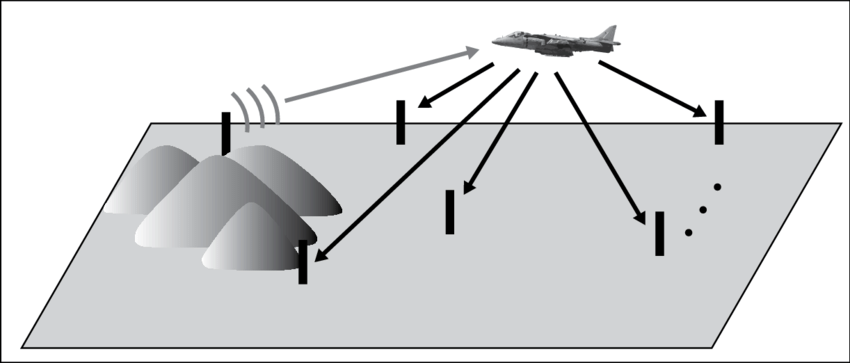
\includegraphics[height=5cm]{multistatic.png}
  \caption{Radar multiestático. Obtido de \cite{mimoradarbook}.}
  \label{fig:multi}
\end{figure}

Este tipo de radar MIMO é designado de não coerente ou estatístico, por razões estudadas mais à frente.

Se, por outro lado, os emissores se encontrarem próximos uns dos outros, possivelmente na mesma plataforma ou agregado, então o sistema é designado de radar MIMO coerente.
Este é a variante mais comum, e a estudada em mais detalhe neste trabalho.

\begin{figure}[h]
  \centering
  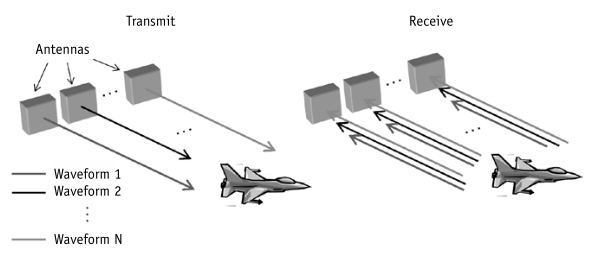
\includegraphics[height=5cm]{concept.png}
  \caption{Radar MIMO coerente. Obtido de \cite{mimoradarbook}.}
  \label{fig:concept}
\end{figure}

\subsection{MIMO coerente e não coerente}

No radar MIMO \textbf{coerente}, a colocação das antenas não difere do radar convencional, tal que as antenas de emissão e receção partilham o ângulo de observação a um alvo distante.
Uma consequência é que a RCS (\textit{radar cross-section}) será praticamente constante.
Este tipo pode ser visto como uma generalização do radar mono-estático, e um esquema é visível na figura \ref{fig:concept}.
\todo[disable]{As fontes estão bué confusas aqui, mas isto é importante}

No radar MIMO \textbf{não coerente}, os transmissores e receptores são necessariamente antenas separadas, colocadas em diferentes posições numa certa área, tal que os ângulos de observação ao alvo são diferentes para cada elemento.

\section{Perspetiva Histórica}

Em telecomunicações, técnicas MIMO são usadas desde os anos 90, pois apresentam um conjunto de vantagens em relação ao tradicional SISO (\textit{Single-Input Single-Output}).
Em primeiro lugar, aumenta a eficiência espectral, isto é, a quantidade de informação transmitida por segundo e por hertz para uma potência fixa. 
Além disso, melhora-se a robustez ao desvanecimento, pela informação poder ser enviada de emissores não correlacionados.

Em contrapartida à metodologia SISO em que se transmite toda a energia num só percurso de comunicação, as comunicações MIMO permitem explorar a diversidade espacial, já que o desvanecimento actua independentemente para cada transmissor.
Assim, o SNR (\textit{Signal-to-Noise Ratio}) no recetor não depende dramaticamente do desvanecimento dos canais individuais.

Em essência, para comunicações em MIMO, a informação transmitida é desconhecida, mas os canais são conhecidos, e até estáticos. Para o radar MIMO, as formas de onda emitidas são conhecidas, mas o ambiente, como a presença de \textit{clutter} ou \textit{jamming}, não o são.

A motivação para o aplicar o conceito MIMO a radares foi mesmo a ideia de diversidade espacial, que permitiria ultrapassar a cintilação dos alvos através de transmissões não correlacionadas.
Contudo, a ideia não se restringe ao uso de vários elementos radiadores.
De facto, agregados de fase \todo{É esta a tradução de phased arrays?} são usados à muito tempo para detectar alvos pequenos a grandes distâncias.
A diferença é que neste caso os sinais de saída só diferem na fase entre si de maneira a guiar um lobo de ganho elevado. 
Estes sinais são então correlacionados e não oferecem mais nenhum grau de liberdade.

\todo[disable]{Mais a ser escrito aqui}

O radar MIMO trata-se de uma tecnologia emergente, com centenas de artigos publicados nos últimos 15 anos, e com o primeiro sistema a aplicar este conceito desenvolvido nos anos 90.
Contudo, é tomado com algum ceticismo, já que o seu uso em certas aplicações degrada substancialmente o desempenho de sistemas convencionais.
As aplicações onde o radar MIMO supera os sistemas convencionais são \textit{airborne surface surveillance} e \textit{Over-The-Horizon radars}.

\section{Radar MIMO}

\subsection{Princípos de comunicações MIMO e radar}

A meta de qualquer sistema de radar é inferir uma propriedade do ambiente a partir das características das ondas eletromagnéticas transmitidas.
Os sistemas de radar são normalmente modelados linearmente, com a entrada sendo o sinal irradiado, e a saída o sinal recebido. 
Para o caso SISO, denomeia-se $x(t)$ a representação complexa do sinal de entrada transportado na frequência $\omega_c$, $(t)$ a saída, $h(t)$ a resposta impulsiva e $v(t)$ o ruído no recetor.
A resposta pode ser dada por:
\begin{align}
  y(t) = \int_0^\infty h(\tau)e^{-i\omega_c\tau}(t-\tau)d\tau + v(t).
  \label{eq:linearsiso}
\end{align}

No caso das telecomunicações, $h(t)$ é função do canal de comunicações, enquanto que para o problema de radar monoestático pode ser chamada de \textit{range profile}.
Para qualquer dos casos, $h(t)$ pode ser construído pelo sinal medido de um certo número de recetores, que chegam com o mesmo atraso $\tau$, mas com diferentes ângulos de chegada $\theta$:
\begin{align}
  h(\tau) = \int_{-\pi}^{\pi}\alpha(\tau,\theta)d\theta.
  \label{eq:profile}
\end{align}
%Para o radar, o objetivo pode ser estimar este par ângulo/atraso.

No caso MIMO, é usado um conjunto de sinais de entrada, $\mathbf{x}(t)\in\mathbb{C}^M$, e um conjunto de sinais de saída, $\mathbf{y}(t)\in\mathbb{C}^N$.
O modelo da equação \ref{eq:linearsiso} pode ser expandido para:
\begin{align}
  \mathbf{y}(t) = \int_0^\infty \mathbf{H}(\tau)e^{-i\omega_C \tau}\mathbf{x}(t-\tau)d\tau + \mathbf{v}(t),
  \label{eq:linearmimo}
\end{align}
onde $\mathbf{H}(t)$ é uma matriz $N\times M$ que descreve a resposta dos $MN$ canais do sistema MIMO.
Os ganhos ao usar MIMO são dependentes da informação adicional dada por $\mathbf{H}$, de facto, se esta for mal condicionada, as vantagens são limitadas. 
Nas telecomunicações, procura-se explorar a diversidade espacial dada pelos $MN$ canais, o que pode ser visto como garantir redundâncias, para pelo menos um caminho esteja disponível.
Aliás, antenas recetoras distanciadas de apenas um comprimento de onda podem receber sinais completamente independentes que transportam informação redundante.

No caso de um radar MIMO coerente e um único alvo, as antenas estão tão perto que observam a mesma reflectividade, e a única diferença será um desvio de fase que está relacionado com o ângulo de incidência.

Embora existam muitas semelhanças entre radar e telecomunicações MIMO, a meta nas comunicações é maximizar SNR no recetor, enquanto que para o radar é optimizar as outras propriedades da antena, eventualmente com o custo de reduzir SNR.
A análise seguinte mostra como o processamento coerente dos sinais de um sistema de radar MIMO pode ser usado para melhorar o desempenho do sistema.

\subsection{Agregado Virtual MIMO}

Um radar MIMO que transmite formas de onda ortogonais pode ser analisado como um agregado virtual.
Trata-se de usar $M$ elementos a transmitir e $N$ elementos usados na recepção, tal que se têm $NM$ elementos virtuais.

Vamos considerar um agregado uni-dimensional, com a posição relativa de cada elemento em relação a um centro arbitrário representada por $x$. 
Adicionalmente, $x_T$ e $x_R$ denotam um elemento transmissor e recetor, respetivamente.
O agregado virtual MIMO correspondente é:
\begin{align}
  \left\{ \frac{x_{Tm}+x_{Rn}}{2}:\; m=1,\ldots,M;\,n=1,\ldots,N \right\}.
  \label{eq:virtualmimo}
\end{align}
Esta construção é feita considerando cada par pseudo-biestático\footnote{O termo pseudo-biestático significa no caso de MIMO coerente que o ângulo biestático é assumido ser pequeno, ie, os elementos transmissores e recetores estão próximos.} entre elementos transmissores e recetores, notando que cada emissor deve utilizar formas de ondas ortogonais.

Na figura \ref{fig:virt1} \emph{a)} observa-se o agregado de fase, em que as formas de onda estão perfeitamente correlacionadas, o que implica existirem $N$ centros de fase.
Na figura \ref{fig:virt1} \emph{b)}, usam-se formas de onda não correlacionadas, o que produz $NM$ centros de fase virtuais, embora não todos distintos.
Se o objetivo for obter um agregado virtual contínuo, tal é possível separando os elementos transmissores, como na figura \ref{fig:virt1} \emph{c)}. 

\begin{figure}[h]
  \centering
  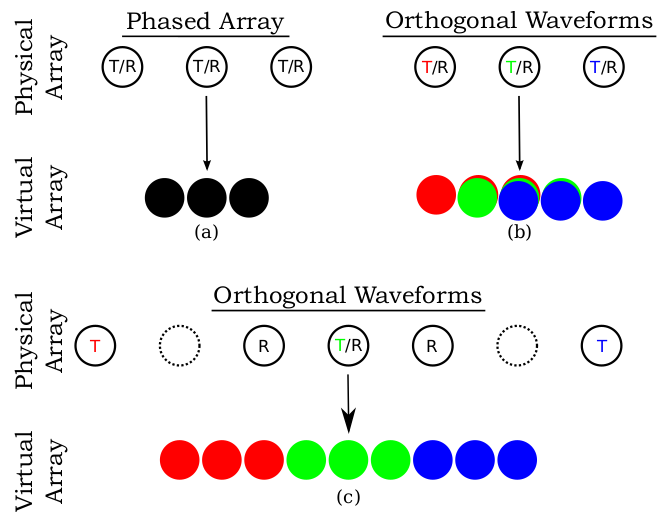
\includegraphics[height=7cm]{virt1.png}
  \caption{Agregados virtuais equivalentes. Obtido de \cite{davis2015mimo}.}
  \label{fig:virt1}
\end{figure}

Como observado, transmitir formas de onda ortogonais origina centros de fase adicionais, o que traz duas vantagens.
Em primeiro lugar, o \textit{spatial sampling rate}\todo{Preciso de tradução disto e talvez incluir uma definição} pode ser aumentado por um fator de $M$ face ao agregado de fase, o que é útil para captação de imagens com abertura sintética.\todo{Verificar esta tradução}
Em segundo, exitem benifícios ao nível da resolução angular quando se aumenta o tamanho do agregado virtual.

\subsubsection{Formas de Onda Ortogonais}

Na presente secção, menciona-se que cada elemento emissor deve usar formas de onda ortogonais entre si, o que pode ser atingido de várias maneiras.
Uma proposta, é usar \textit{spectrally interleaved multi-carrier system} de \cite{sturm2013spectrally}, onde cada \textit{subcarrier} é distribuída em antenas espaçadas.
As formas de onda são ortogonais para este método se 
\begin{align}
  f_n = n\Delta f = \frac{n}{T}, \; n=0,\ldots,N_c -1,
  \label{eq:orth}
\end{align}
onde $f_n$ são as frequências de \textit{subcarriers}, $T$ é a duração de símbolo de OFDM \footnote{Orthogonal fequency-division multiplexing}, e $N_c$ o número de \textit{subcarriers}.

Outro método é usar um sinal \textit{chirp} ortogonal de \cite{chen2008mimo}, expresso como
\begin{align}
  x_m(t)= exp\left( 2\pi \left( f_{m,0}t+\frac{1}{2}kt^2 \right) \right).
  \label{eq:chirp}
\end{align}
Os sinais podem ser tornados ortogonais escolhendo adequadamente $f_{m,0}$ e $k$.

\todo[inline]{Subsecção sobre coarray, se me apetecer}

\section{Processamento de Sinais para radar MIMO}

Considere-se um radar MIMO que transmite $M$ formas de onda independentes, possivelmente de vários elementos emissores, ou de agregados, desde que cada sinal tenha um centro de fase distinto.
Os sinais são refletidos no ambiente e observados por $N$ recetores, que podem ou não ser os mesmos usados na transmissão.
Este caso está esquematizado na figura \ref{fig:rad3}.

\begin{figure}[hp]
  \centering
  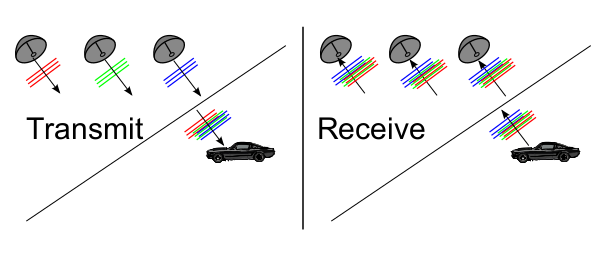
\includegraphics[width=0.8\linewidth]{rad3.png}
  \caption{Modelo de um radar MIMO com $N=M=3$. Obtido de \cite{davis2015mimo}.}
  \label{fig:rad3}
\end{figure}

Com algumas assumpções,\todo{Especificar?} pode admitir-se que os sinais observados por cada elemento são idênticos a menos de um desvio em fase.
Seja $x_m(t)$ o sinal emitido pelo elemento $m$ e $y_n$ o sinal observado no elemento $n$, de um alvo com ângulo $\theta_0$, então pode escrever-se:
\begin{align}
  y_n(t,\theta) = \alpha b_n(\theta_0) \sum_{m=1}^{M}a_m(\theta_0)x_m(t) + v_n(t),
  \label{eq:proc1}
\end{align}
onde $\alpha$ é um coeficiente de \textit{backscatter}, $a_m$ e $b_n$ são os desvios de fase na transmissão e recepção, respetivamente.

Estes desvios de fase podem ser tratados como vetores $\mathbf{a} \in \mathbb{C}^M$ e $\mathbf{b} \in \mathbb{C}^N$.
Assim, a equação \ref{eq:proc1} toma uma forma mais compacta:
\begin{align}
  \mathbf{y}(t,\theta_0) = \alpha\mathbf{b}(\theta_0)\mathbf{a}(\theta_0)^T\mathbf{x}(t)+\mathbf{v}(t).
  \label{eq:radc}
\end{align}
A interpretação de que os sinais recebidos por um radar MIMO são a combinação linear dos sinais transmitidos leva à definição de $\mathbf{H}$ como
\begin{align}
  \mathbf{H}(\theta) \coloneqq \mathbf{b}(\theta)\mathbf{a}(\theta)^T,
  \label{eq:H}
\end{align}
que depende explicitamente do ângulo $\theta$.

Um radar MIMO aplica filtros adaptados, com a hipótese comum de todas as formas de onda serem ortogonais, o que implica que cada filtro vai seleccionar um e um só sinal, descartando o resto.
Cada recetor terá $M$ destes filtros, o que é visível na figura \ref{fig:proc} ainda para o caso $M=N=3$.

\begin{figure}[ht]
  \centering
  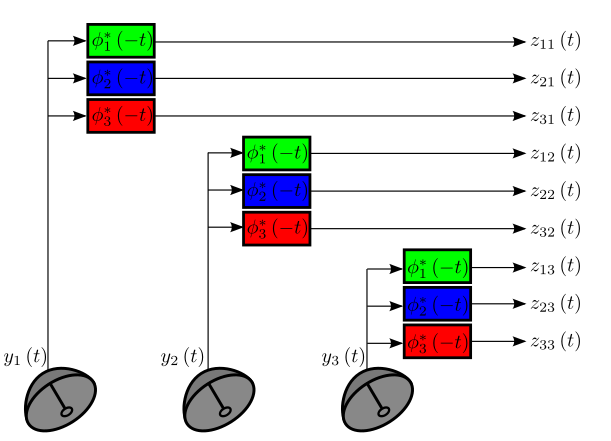
\includegraphics[height=7cm]{processor.png}
  \caption{Processamento de sinais em radar MIMO. Obtido de \cite{davis2015mimo}.}
  \label{fig:proc}
\end{figure}

O resultado desta filtragem é a matriz $N\times M$:
\begin{align}
  \begin{aligned}
    \mathbf{Z}(\theta_0) &= \int_{-\infty}^{\infty} \mathbf{y}(t,\theta_0)\mathbf{x}(t)^Hdt \\
	&= \alpha \mathbf{H}(\theta_0)\mathbf{R}_x + \mathbf{E} ,
  \end{aligned}
  \label{eq:Z}
\end{align}
com $\mathbf{R}_x$ a matriz de correlação dos sinais de entrada e $\mathbf{E}$ o ruído no filtro.

Pode ser mostrado que o $SNR$ obtido com este processamento é inferior ao do radar convencional por um fator de $\frac{1}{M^2}$, (ver figura \ref{fig:tabela} de \cite{mimoradarbook}), o que deve ser compensado com processamento coerente.
Com este, usando um \textit{threshold} $\gamma$, a saída do filtro terá uma distribuição gaussiana com média nula, e a deteção um distribuição exponencial, de onde seguem as probabilidades de deteção e falso alarme:
\begin{align}
  p_d &= exp\left( -\frac{\gamma}{\sigma_t^2 + \sigma_n^2} \right) \label{eq:pd} \\
  p_{fa} &= exp\left( -\frac{\gamma}{\sigma_n^2} \right) \label{eq:pfa},
\end{align}
onde $\sigma_t^2$ e $\sigma_n^2$ são as potências do alvo e interferência (\textit{clutter} mais ruído), respetivamente.

\begin{figure}[ht]
  \centering
  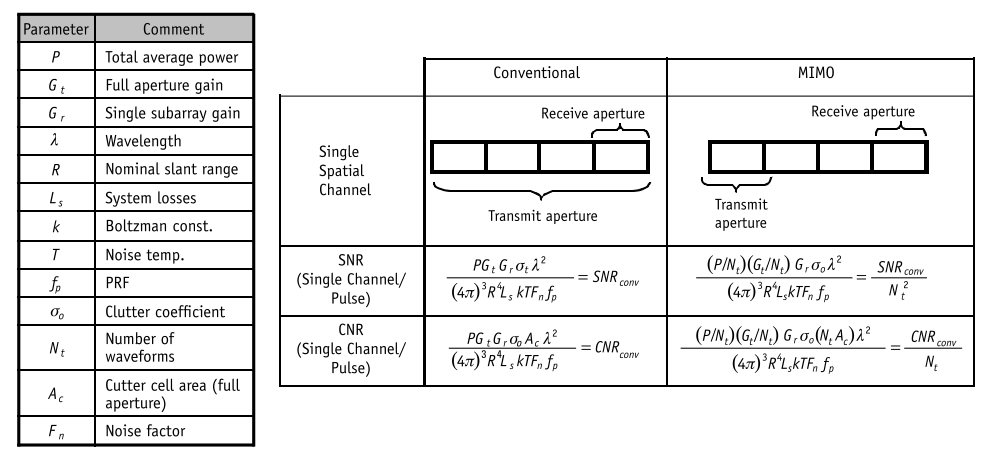
\includegraphics[width=\linewidth]{table.png}
  \caption{Comparação da sensibilidade do radar MIMO e convencional. Obtido de \cite{mimoradarbook}.}
  \label{fig:tabela}
\end{figure}

\section{Exemplos de Aplicações}

\subsection{Aplicação a Sistemas de Imagens por Radar}

A captação de imagens de grandes superfícies geográficas de alta resolução é um campo de elevada relevância e dificuldade devido à escala considerada e a atenuação óptica da atmosfera para grandes distâncias e altitudes necessárias para captação eficiente das superfícies mencionadas.

Desde cedo se relevou uma aplicação útil da tecnologia radar. Colocando radares a altitudes elevadas para o propósito, os sinais emitidos são refletidos pela superfície terrestre e são captados pelo radar com propriedades diferentes dependendo da superfície atingida, permitindo ao radar obter informação sobre a composição de determinadas zonas captadas no seu alcance.

\begin{figure}[ht]
	\centering
	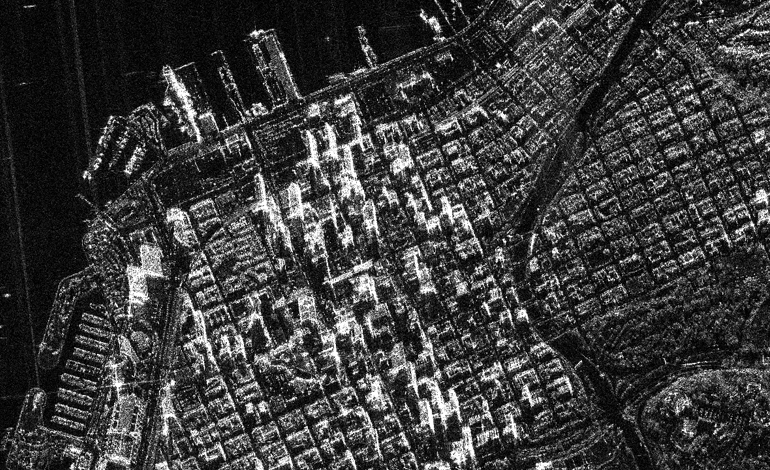
\includegraphics[width = 0.7\textwidth]{sandiego}
	\caption{Exemplo de imagem obtida por radar, através de SAR.}
	\label{fig:sandiego}
\end{figure}

Em comparação a fotografia óptica, que para a escala considerada tem o seu alcance diminuído não só por obstáculos atmosféricos como nuvens, tempestades, ou outros fenómenos meteorológicos, como também pela composição da atmosfera em si, os sinais de rádio emitidos por radares são muito menos afetados por este tipo de interferências.

Devido a estas vantagens, a criação de imagens de grandes superfícies e a sua aplicação em mapeamento terrestre, monitorização ambiental e sistemas de reconhecimento militar é frequentemente auxiliada por sistemas de radares próprios para o efeito.

\subsubsection{Radar de Abertura Sintética}

O \textsc{Radar de Abertura Sintética}, doravante referido pela sigla inglesa SAR, é um sistema de radar aéreo ou espacial que beneficia do seu movimento para obter vários sinais diferentes ao longo da sua trajetória, juntando-os para criar um resultado final, utilizando os sinais obtidos como referências espaciais diferentes, como se pode verificar na figura \ref{subfig:sar-timesteps}.

\begin{figure}[ht]
	\centering
	\hspace*{\fill}
	\begin{minipage}[t]{0.43\textwidth}
		\centering
		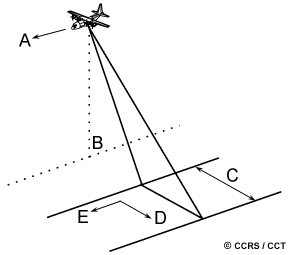
\includegraphics[height=4cm]{radgeom}
		\subcaption{Esquema geral do uso de SAR. Na imagem os rótulos representam \figlabel{A} a trajetória de voo, \figlabel{B} o \textit{nadir}, \figlabel{C} a faixa iluminada a cada instante, \figlabel{D} o alcance a cada instante e \figlabel{E} a zona iluminada prevista na trajetória.}
		\label{subfig:sar-side}
	\end{minipage}
	\hfill
	\begin{minipage}[t]{0.43\textwidth}
		\centering
		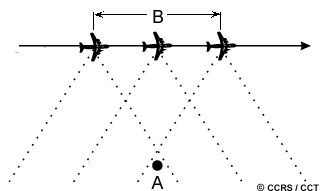
\includegraphics[height=4cm]{sar}
		\subcaption{Captação de imagens em movimento são utilizadas como perspetivas diferentes. Quando um alvo \textbf{A} entra no alcance do radar, inicia-se o cálculo da distância entre antenas simuladas \textbf{B}, que é o segmento máximo da trajetória em que \textbf{A} se encontra em alcance.}
		\label{subfig:sar-timesteps}
	\end{minipage}
	\hspace*{\fill}
	\caption{Ilustrações sobre o SAR, cortesia da \textit{Natural Resources Canada} \cite{nrcan}.}
	\label{fig:nrcan}
\end{figure}

O radar é contido num veículo que se encontra em voo a alta velocidade, a uma altitude moderada que depende da escala da área a ser mapeada. O radar emite pulsos ao longo do deslocamento e recebe ecos suficientes para construir uma imagem do ambiente à sua volta a cada instante.

Acrescentando-lhe informação do movimento, o radar consegue aumentar a definição do mapeamento ao longo da direcção indicada por \figlabel{E} na figura \ref{subfig:sar-side}. Dado a que utiliza vários pontos de vista diferentes para o mesmo alvo, e a elevada quantidade de imagens retiradas, o alcance individual de cada imagem pode ser mais reduzida para depois ser composta com as imagens restantes para formar uma imagem com maior alcance. A frequência de obtenção destas imagens, doravante referido por \textit{sampling rate}, necessita de ser grande o suficiente para adquirir dados de toda a superfície sem deixar falhas no mapeamento.

Comparando uma colecção de sinais de SAR obtidos a uma matriz de antenas uniformemente espaçadas, podemos utilizar o valor de $B$ da figura \ref{subfig:sar-timesteps} como a distância entre as antenas da matriz. Assim, pelo critério de Nyquist, esta distância não pode ser superior a metade da frequência do sinal utilizado, ou seja, $B \leq \lambda/ 2$, para evitar ambiguidades nos sinais recebidos.

O sistema transmite pulsos a uma frequência $f_p$ a uma velocidade de movimento $v$ constante. Assim, podemos determinar o intervalo de \textit{sampling} espacial, ou a distância viajada entre pulsos, como $\delta_x$.
\begin{gather*}
	\delta_x \triangleq \frac{v}{f_p}
\end{gather*}
O SAR tem de ter uma frequência elevada o suficiente para ter uma resolução da imagem aceitável, mas não grande demais para ter uma razão de área por \textit{sample} também considerável. Esta razão, referida por ACR (do inglês \textit{Area-Coverage Rate}, pode ser calculada para uma plataforma a movimentar-se a uma velocidade constante, utilizando a velocidade e a largura na direcção ortogonal \figlabel{D} na figura \ref{subfig:sar-side} de uma imagem, rotulada de $R_{\textrm{swath}}$.
\begin{gather*}
	ACR \triangleq vR_{\textrm{swath}}
\end{gather*}
O valor de $R_{\textrm{swath}}$ está limitado pela velocidade de transmissão de pulsos $f_p$. Assim, o valor de $ACR$ também está limitado.
\begin{gather*}
	R_{\textrm{swath}} < \frac{c/2}{f_p} \\
	ACR < \delta_x\left(\frac{c}{2}\right)
\end{gather*}

A frequência $f_p$ é tanto melhor quanto menor for o seu valor, para maximizar o valor de $ACR$. No entanto, ainda é desejada uma resolução de imagem razoável, pelo que a frequência não pode ter um valor demasiado reduzido. Aumentando a abertura do radar resolve este problema ao adquirir mais dados por \textit{sample}, mas este método pode distorcer a qualidade das imagens devido a ângulos de incidência maiores.

Outra solução passa pela implementação de mais recetores, que significa que múltiplos \textit{samples} são recebidos por cada pulso enviado. Comparando mais uma vez os sinais recebidos ao longo da trajetória de voo a um \textit{array} com distância $D$ entre os seus componentes, para $N$ recetores, a distância entre emissões passará a ser $N \cdot D$. Assim, a frequência de \textit{sampling} pode ser aumentada sem aumentar a frequência de emissão $f_p$.

Este sistema pode ser conisderado \textit{Single-Input Multiple-Output}, mas pode ser extendido a MIMO ao utilizar vários emissores com formas de onda diferentes.

\subsection{Radar Automóvel}

Radares automóveis estão a entrar rapidamente no mercado, tanto no aumento de segurança e conveniência do condutor como na aplicação a automóveis autónomos. Face a outros métodos semelhantes como câmeras, \textit{lidar} e \textit{sonar}, as vantagens são semelhantes a outras já referidas, como viabilidade em condições meteorológicas adversas. No entanto, radares MIMO estão a ganhar terreno sobre outros radares devido ao seu custo mais reduzido.

\begin{figure}[ht]
	\centering
	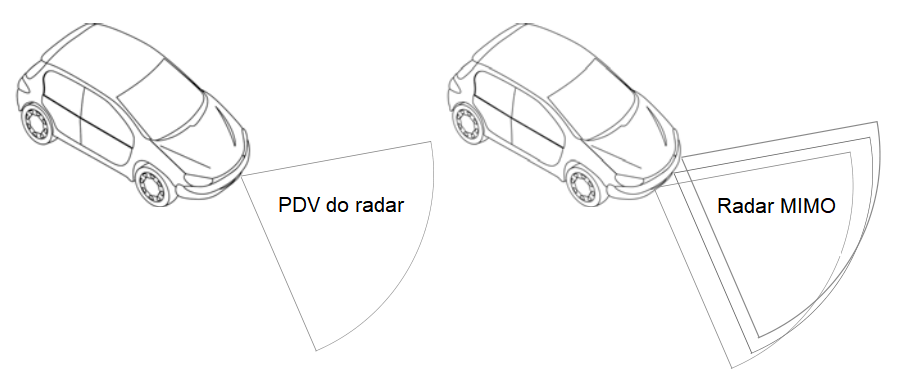
\includegraphics[width=0.7\textwidth]{auto}
	\caption{Radar automóvel dianteiro \textit{standard} (à esquerda), onde PDV significa ponto de vista, e utilizando MIMO (à direita). Obtido de \textit{\citeauthor{mimoradarbook}} \cite{mimoradarbook}.}
	\label{fig:autorad}
\end{figure}

O radar automóvel da figura \ref{fig:autorad} representa uma aplicação de radar. A detecção de distâncias a obstáculos dentro do ponto de vista do radar e a sua velocidade revela ser relativamente simples mesmo com radares SISO. No entanto, obter o ângulo de obstáculos pode ser uma dificuldade com este tipo de radar.

Embora utilizar sistemas como \textit{phased arrays} possa ser uma solução, a aplicação com sistemas de tamanho mais reduzido como o utilizado aqui favorece os radares MIMO pelo custo. Vários emissores alinhados entre si cobrem cada um uma abertura reduzida, e todas as aberturas se sobrepõem para cobrir uma área de interesse. Um recetor centrado recebe todos os sinais e filtra-os separadamente para identificar o espaço à sua frente.

Em comparação a um \textit{phased array}, um radar MIMO consegue obter um resulado similar sem recorrer a mudanças de fase ou canais de frequência separados. No entanto, resulta num SNR menor.

\subsection{Radar Além-Horizonte}

Uma técnica de radar conhecida por radar além-horizonte, ou \textit{Over-The-Horizon}, doravante referido por OTH, utiliza as diferentes altitudes das várias camadas da ionosfera terrestre para obter respostas de distâncias muito superiores ao alcance direto do radar, podendo assim ultrapassar a curvatura da terra, aumentando bastante o alcance do radar.

No entanto, o uso extensivo da atmosfera como modo de propagação implica o acréscimo de ruído e \textit{clutter}, e perdas de sinal muito maiores devido às reflexões adicionais para obter um sinal. Estes problemas dificultam bastante a detecção e reduzem imenso a resolução da resposta.

\begin{figure}[ht]
	\centering
	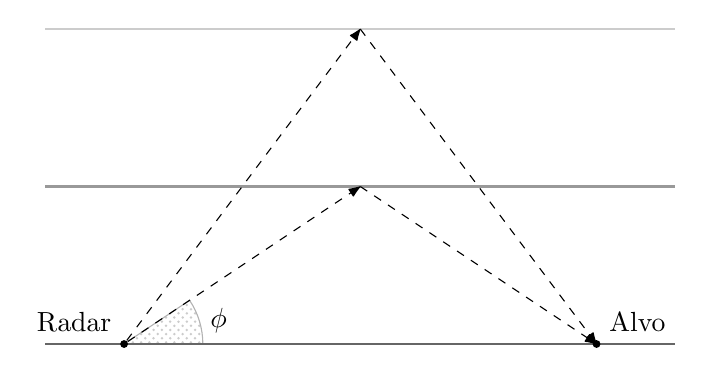
\begin{tikzpicture}[]
		\path [pattern = crosshatch dots, pattern color = white!80!black,draw=white!70!black] (1,0) -- ++(1,0) arc (0:33.69:1) -- cycle;
		\node at (2.2,0.3) [] {$\phi$};
		\path [draw=white!40!black,thick] (0,0) -- (8,0);
		\path [draw=white!60!black,thick] (0,2) -- (8,2);
		\path [draw=white!80!black,thick] (0,4) -- (8,4);
		\node (radar) at (1,0) [circle,fill,inner sep = 1pt,label={135:Radar}] {};
		\path [draw,-{Latex[round]},dashed] (radar) -> (4,2);
		\path [draw,-{Latex[round]},dashed] (4,2) -> (7,0);
		\path [draw,-{Latex[round]},dashed] (radar) -> (4,4);
		\path [draw,-{Latex[round]},dashed] (4,4) -> (7,0);
		\node (target) at (7,0) [circle,fill,inner sep = 1pt,label={45:Alvo}] {};
	\end{tikzpicture}
	\caption{Exemplificação das reflexões atmosféricas e múltiplos trajetos para o alvo com radar OTH.}
	\label{fig:oth}
\end{figure}

Não só existem estes problemas como também pode ocorrer interferência do mesmo sinal através de trajetos diferentes para o mesmo alvo, como exemplificado na figura \ref{fig:oth}. Isto resulta no mesmo sinal a ser recebido com ângulos de envio e receção diferentes.

Quando o \textit{clutter} viaja com ângulos de incidência e receção diferentes do sinal de ilumniação, é possível colocar um anulador de transmissão no ângulo do \textit{clutter} para melhorar a deteção do alvo. No entanto, os ângulos envolvidos neste cálculo não são conhecidos antes da transmissão, pelo que colocar o anulador nem sempre garante melhoria.

Utilizando um radar MIMO o anulador de transmissão pode ser ajustado de acordo com a distância ao alvo, pelo que a deteção é melhorada a todas as distâncias dentro do alcance do radar.

\section{Dificuldades de Implementação}

A implementação de radar MIMO coerente traz alguns desafios, que podem ou não ditar a impossibilidade de usar este sistema. 
Os mais estudados são o aumento da complexidade de computação (em processamento digital), a rejeição adaptativa do \textit{clutter}, e outros problemas de calibração e \textit{hardware}.
Nesta secção discute-se conceptualmente os primeiros dois, e mencionam-se estratégias de mitigação.

\subsection{Complexidade de Computação}

As tarefas de processamento principais em radar são:
\begin{itemize}
  \item Compressão de pulsos
  \item Processamento de Doppler
  \item Rejeição de \textit{clutter}.
\end{itemize}

Para o efeito de analizar a complexidade computacional, os primeiros dois passos são considerados parte de pré-processamento.
A equação \ref{eq:ops_pre} revela a fração de FLOPS\footnote{\textit{floating point operations per second}} quando se usa um radar MIMO com $M$ formas de onda, $N$ recetores e $L$ \textit{bins} no alcance.
\begin{align}
  f_{pre}=1+\frac{\log_2 N}{\log_2 (LM)}.
  \label{eq:ops_pre}
\end{align}
Para chegar a esta expressão, modela-se que a compressão de pulsos é feita com convolução com FFT, e o processamento de doppler também com FFT.
Este fator é pequeno, por exemplo para $N=4$, $M=128$ e $L=1000$, observa-se um aumento de apenas \SI{12}{\percent}. 

Já para a parte da rejeição do \textit{clutter}, a fracção é:
\begin{align}
  f_{STAP} = M\left( \frac{MN^3+L}{M^2N^2+L} \right),
  \label{eq:ops_cl}
\end{align}
e tipicamente, $L$ é muitas vezes superior a $M$ ou $N$, logo o aumento é proporcional ao número de formas de onda.
Isto mostra que no mínimo temos o dobro da carga computacional ao usar MIMO, o que para algumas aplicações é proibitivo. 

\subsection{Rejeição Adaptativa do \textit{clutter}}

Para além do aumento da computação necessária para a rejeição do \textit{clutter}, o aumentado número de graus de liberdade também complica o próprio porcesso no caso de \textit{clutter} heterogéneo. 
Normalmente, a eliminação do \textit{clutter} é feita usando \textit{training data} na dimensão do alcance, e geralmente devem usar-se um número de amostras na ordem dos graus de liberdade, o que se torna ainda mais difícil com o aumento de formas de onda distintas.

As soluções com melhor potencial involvem usar conhecimento \emph{a priori} do ambiente de \textit{clutter} para remover qualquer tendência antes do processamento adaptativo, são chamadas de \textit{knowledge-aided space-time adaptative processing}, KA-STAP.

\section{Conclusões}

O radar MIMO coerente é a extensão natural do agregado de fase, e uma área onde muita investigação está a ser feita, com o objetivo de melhorar a mesma.
No entanto, não é a solução mágica que irá beneficiar todos os sistemas nas suas diversas aplicações. De facto, o desempenho de muitos sistemas é piorado ao usar MIMO, especialmente quando este é limitado pelo ruído de temperatura.
Quando o desempenho é limitado por outros fatores, como o ruído multiplicativo em SAR, \textit{clutter} em GMTI\footnote{Ground Moving Target Indication}, fenómenos na ionosfera, ou problemas de sincronização associada à fusão de dados em radar multiestático, então o radar MIMO pode trazer melhorias.






\nocite{radarhandbook,radarsystems,davis2015mimo,li2018mimo,radartutorial,sturm2013spectrally,chen2008mimo,nrcan,mimoradarbook}
\printbibliography

\listoftodos
\end{document}
